\section{Оценка смещения по методу складного ножа}

Складной нож был оригинальным компьютерным методом оценки смещения и стандартных ошибок. Оценка смещения методом складного ножа, которая кратко обсуждается здесь и более подробно в главе 11, была предложена Морисом Кенуйем в середине 1950-х годов. При наличии набора данных $x = (x_1, x_2, \dots, x_n)$, $i$-я реализация складного ножа $x_{(i)}$ определяется как $x$ с удаленной $i$-й точкой наблюдений,
\begin{equation}\label{eq10.28}
    x_{(i)} = (x_1, x_2, \dots, x_{i-1}, x_{i+1}, \dots, x_n),
\end{equation}
для $i = 1, 2, \dots, n$. Для статистики $\theta = s(x)$ $i$-я репликация складного ножа $\hat{\theta}_{(i)}$~---~это $s(\cdot)$, вычисленная для $x_{(i)}$, предположим
\begin{equation}\label{eq10.29}
    \hat{\theta}_{(i)} = s(x_{(i)}) \quad\quad \text{для}\; i = 1, 2, \dots, n.
\end{equation}
Для статистики метода подстановки $\hat{\theta} = t(\hat{F})$, $\hat{\theta}_{(i)}$ равна $t(\hat{F}_{(i)})$, где $\hat{F}_{(i)}$ --- эмпирическое распределение $n-1$ точек в $x_{(i)}$·

Оценка смещения складного ножа определяется как
\begin{equation}\label{eq10.30}
    \widehat{\text{bias}}_{\text{jack}} = (n-1)\left(\hat{\theta}_{(\cdot)} - \hat{\theta}\right),
\end{equation}
где
\begin{equation}\label{eq10.31}
    \hat{\theta}_{(\cdot)} = \sum\limits_{i=1}^{n}\hat{\theta}_{(i)}/n.
\end{equation}
Эта формула применяется только к статистике метода подстановки $\hat{\theta} = t(\hat{F})$. Формула не работает, если $t(\hat{F})$ --- негладкая статистика, такая как медиана, но для гладкой статистики, такой как $\hat{\theta} = \bar{y}/\bar{z}$ (тех статистик, для которых функция $T(P^{*})$ в (\ref{eq10.20}) дважды дифференцируема) она дает оценку смещения с помощью всего $n$ повторных вычислений функции $t(\cdot)$. Это сравнивается с $B$ повторными вычислениями для будстреп оценок, где $B$ должно быть не менее $200$ даже для $\overline{\text{bias}}_{B}$.

\noindent
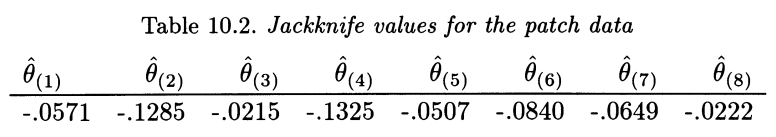
\includegraphics[width=\linewidth]{10/t10.2.png}
\newline

Для данных об уровне гормона статистика отношения $\hat{\theta} = \bar{z}/\bar{y} = -0.0713$ (формула (\ref{eq10.10})), репликации складного ножа показаны в таблице 10.2. Это приводит к $\hat{\theta}_{(\cdot)} = -0.0702$, и
\begin{equation}\label{eq10.32}
    \widehat{\text{bias}}_{\text{jack}} = 7\{-0.0702 - ( -0.0713)\} = 0.0080.
\end{equation}
Не случайно, что $\widehat{\text{bias}}_{\text{jack}}$ так близко согласуется с идеальной бутстреп оценкой $\widehat{\text{bias}}_{\infty} = \widehat{\text{bias}}_{\hat{F}}$. В главе 20 показано, что $\widehat{\text{bias}}_{\text{jack}}$ --- это приближение оценки смещения, полученной по методу подстановки, рядом Тейлора второго порядка. Важно помнить следующее: все три оценки смещения, $\widehat{\text{bias}}_{B},\, \overline{\text{bias}}_{B}$ и $\widehat{\text{bias}}_{\text{jack}}$ пытаются аппроксимировать одну и ту же идеальную оценку $\text{bias}_{\hat{F}}$. В главе 20 обсуждается инфинитезимальный складной нож --- еще один способ приблизительного определения смещения. Мы также увидим аппроксимации, отличные от $\widehat{\text{se}}_{B}$, для идеальной оценки стандартной ошибки $\text{se}_{\hat{F}}$ (хотя здесь сложнее улучшить прямое приближение Монте-Карло $\widehat{\text{se}}_{B}$). Во всех методах численной аппроксимации работает только один принцип оценки, подстановка $\hat{F}$ вместо $F$ в любую меру точности, которую мы хотим оценить. Реализация этого принципа численно эффективным способом --- важная тема, но современные компьютеры настолько мощны, что даже неэффективные способы обычно достаточно хороши, чтобы дать пригодные ответы.

Идеальная оценка $\text{bias}_{\hat{F}}$ имеет недостатки. Если позволить $B \rightarrow \infty$, изменчивость смещения $\widehat{\text{bias}}_{B}$ из-за выборки Монте-Карло устраняется. Однако остается вариабельность $\widehat{\text{bias}}_{\infty} = \text{bias}_{\hat{F}}$ из-за случайности $\hat{F}$ как оценки $F$. Другими словами, у нас все еще есть обычные ошибки, связанные с оценкой любого параметра по выборке.

\noindent
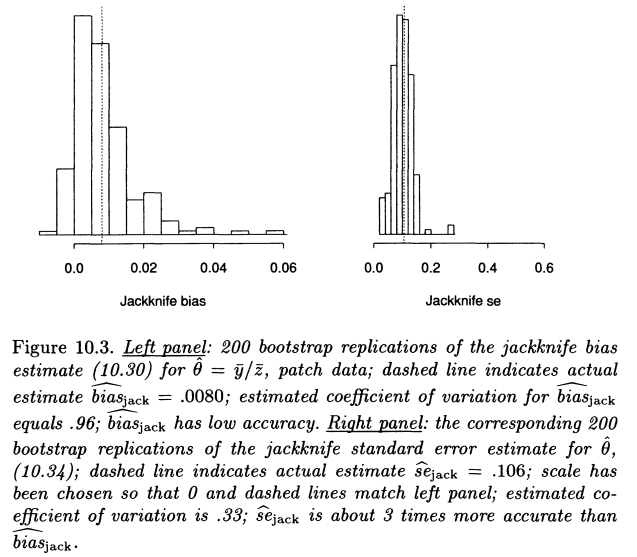
\includegraphics[width=\linewidth]{10/f10.3.png}

Мы могли бы использовать бутстреп для вычисления изменчивости идеальной бутстреп оценки $\text{bias}_{\hat{F}}$, как показано на рисунке 6.1, за исключением практических трудностей вычисления статистики $s(x) = \text{bias}_{\hat{F}}$. Вместо этого давайте рассмотрим более простую статистику $s(x) = \widehat{\text{bias}}_{\text{jack}}$, которая для $\hat{\theta} = \bar{y}/\bar{z}$ обычно близка к $\text{bias}_{\hat{F}}$. Статистика $s(x) = \widehat{\text{bias}}_{\text{jack}}$ является сложной функцией от $x$, требующей сначала вычисления $\hat{\theta}$, затем $\hat{\theta}_{(i)}$ и, наконец, (\ref{eq10.30}), но мы все ещё можем использовать бутстреп для оценки стандартной ошибки $s(x)$.

$B = 200$ бутстреп выборок размера $n = 8$ были сгенерированы из данных об уровне гормона при ношении пластырей, и для каждой выборки была рассчитана оценка смещения по методу складного ножа для статистики отношения, скажем, $\widehat{\text{bias}}_{\text{jack}}^{*}$. Левая часть рисунка 10.3 представляет собой гистограмму из $200$ значений $\widehat{\text{bias}}_{\text{jack}}^{*}$.

Ясно, что статистика $s(x) = \widehat{\text{bias}}_{\text{jack}}$ сильно варьируется. Стандартное отклонение и среднее $200$ репликаций $s(x^{*})$ равнялись соответственно $0.0081$ и $0.0084$, что давало оценку коэффициента вариации 
\begin{equation}\label{eq10.33}
    \widehat{\text{cv}}(\widehat{\text{bias}}_{\text{jack}}) = 0.0081/0.0084 = 0.96.
\end{equation}
Десять процентов значений $\widehat{\text{bias}}_{\text{jack}}^{*}$ были меньше нуля и $16\%$ больше $2\cdot \widehat{\text{bias}}_{\text{jack}} = 0.0160$.

Нет ничего плохого ни в $\widehat{\text{bias}}_{\text{jack}}$, ни в $\text{bias}_{\hat{F}}$. Проблема в том, что $n = 8$ точек данных недостаточно для точного определения смещения статистики отношения в этой ситуации. Рисунок 10.3 поясняет это. Вычисления смещения не были пустой тратой времени. Мы достаточно уверены, что истинное смещение $\hat{\theta} = \bar{y}/\bar{z}$ , каким бы оно ни было, находится где-то между $-0.005$ и $0.025$. Бутстреп стандартная ошибка $\hat{\theta}$ была $0.105$, поэтому отношение абсолютного смещения к стандартной ошибке, вероятно, меньше $0.25$. Вычисление (\ref{eq10.14}) показывает, что в данном случае систематическая ошибка не вызывает особого беспокойства.

Этот расчет предполагает другое беспокойство. Возможно, бутстреп оценка стандартной ошибки $\widehat{\text{se}}_{200} = 0.105$ тоже ненадежна. Теоретически мы могли бы провести бутстреп $\widehat{\text{se}}_{200}$, чтобы выяснить это, но это сложно с вычислительной точки зрения. Однако существует оценка стандартной ошибки по методу складного ножа, предложенная Джоном Тьюки в конце 1950-х годов, которая требует меньше вычислений, чем $\widehat{\text{se}}_{200}$:
\begin{equation}\label{eq10.34}
    \widehat{\text{se}}_{\text{jack}} = \left[\frac{n-1}{n}\sum\limits_{i=1}^{n}\left(\hat{\theta}_{(i)} - \hat{\theta}_{(\cdot)}\right)^{2}\right]^{1/2}.
\end{equation}
Эта формула, которая применяется к гладко определенной статистике, такой как $\hat{\theta} = \bar{y}/\bar{z}$, обсуждается в главе 11. Оказывается, это альтернатива $\widehat{\text{se}}_{B}$ численной аппроксимации идеальной бутстреп оценки $\widehat{\text{se}}_{\infty} = \text{se}_{\hat{F}}(\hat{\theta}^{*})$. Статистика отношения данных об уровне гормона (\ref{eq10.2}) дает
\begin{equation}\label{eq10.35}
   \widehat{\text{se}}_{\text{jack}} = 0.106,
\end{equation}
почти то же самое, что и $\widehat{\text{se}}_{200}$. Мы увидим, что $\widehat{\text{se}}_{\text{jack}}$ не всегда является хорошим приближением к $\widehat{\text{se}}_{\infty}$, но для $\hat{\theta} = \bar{y}/\bar{z}$ это вполне приемлемо.

Те же $200$ бутстреп выборок, использованные для обеспечения репликации $\widehat{\text{bias}}_{\text{jack}}$ на рисунке 10.3, также дали бустреп репликации $\widehat{\text{se}}_{\text{jack}}$. Гистограмма $200$ бутстреп значений  $\widehat{\text{se}}_{\text{jack}}$, показанная на правой части рисунка 10.3, указывает на существенную изменчивость, но не такую большую, как для $\widehat{\text{bias}}_{\text{jack}}$. Гистограмма имеет среднее значение $0.099$ и стандартное отклонение $0.033$, что дает выборочный коэффициент вариации
\begin{equation}\label{eq10.36}
   \widehat{\text{cv}}(\widehat{\text{se}}_{\text{jack}}) = 0.33,
\end{equation}
только треть $\widehat{\text{cv}}(\widehat{\text{bias}}_{\text{jack}})$. На самом деле стандартную ошибку обычно легче оценить, чем смещение, а также она является более важным фактором, определяющим вероятностные характеристики оценки $\hat{\theta}$.

Мы обсудили оценку $\text{bias}_{F}(\hat{\theta}, \theta)$, уравнение (\ref{eq10.1}). Бутсреп процедуру оценки смещения, которая сводится к подстановке $\hat{F}$ вместо $F$ в $\text{bias}_{F}$, можно обобщить: 1) мы можем рассмотреть общие вероятностные механизмы $P \rightarrow x$, как на рисунке 8.3. (Обратите внимание, что здесь <<$P$>> означает нечто иное, чем вектор повторной выборки $P^{*}$, (\ref{eq10.18}).) 2) Мы можем рассмотреть общие меры смещения, $\text{bias}_{P}(\hat{\theta}, \theta)$, например, медианное смещение
\begin{equation}\label{eq10.37}
   \text{bias}_{P}(\hat{\theta}, \theta) = \text{median}_{P}(\hat{\theta}(x)) - \theta(P).
\end{equation}
На рисунке 10.4 показана схема. Идеальная бутстреп оценка $\text{bias}_{P}(\hat{\theta}, \theta)$ это оценка метода подстановки
\begin{equation}\label{eq10.38}
   \text{bias}_{P}(\hat{\theta}^{*}, \theta(\hat{P})).
\end{equation}
Здесь $\hat{P} \rightarrow x^{*}$ --- бутстреп данные; $\hat{\theta}^{*} = s(x^{*})$ --- бутстреп репликация $\hat{\theta} = s(x)$; и $\theta(\hat{P})$~---~значение интересующего параметра $\theta = t(P)$, когда $P=\hat{P}$, механизм оценки вероятности. (Мы не можем писать $\theta(\hat{P}) = \hat{\theta}$, поскольку $t(\cdot)$ может быть другой функцией, отличной от $s(\cdot)$) Для медианного смещения (\ref{eq10.37})
\begin{equation}\label{eq10.39}
   \text{bias}_{\hat{P}}(\hat{\theta}^{*}, \theta(\hat{P})) = \text{median}_{\hat{P}}(\hat{\theta}(x^{*})) - \theta(\hat{P}).
\end{equation}
Обычно $\text{bias}_{\hat{P}}$ нужно аппроксимировать методами Монте-Карло. Усовершенствованные методы, такие как $\overline{\text{bias}}_{B}$ и $\widehat{\text{bias}}_{\text{jack}}$, обычно недоступны для общих мер смещения, таких как (\ref{eq10.37}).